\documentclass[aspectration=1610,t]{beamer}

\usepackage{mooc}

\title{{\bf Программирование на языке \langcpp\protect\\Лекция
7\protect\vspace{1em}\\}Множественное наследование}

\begin{document}
\begin{frame} 
  \titlepage
\end{frame}

% % % % % % % % % % % % % % % % % % % % % % % % % % % % % % % % %
\begin{frame}[fragile]{Множественное наследование}
    \emph{Множественное наследование (multiple inheritance)}~--- возможность
    наследовать сразу несколько классов.
\medskip
    \begin{lstlisting}
struct Unit {
    Unit(unitid id, int hp): id_(id), hp_(hp) {}
    virtual unitid id() const { return id_; }
    virtual int    hp() const { return hp_; }
private:
    unitid id_;
    int	   hp_;
};

struct Elf:    Unit { ... };
struct Archer: Unit { ... };

struct ElfArcher: Elf, Archer {
    unitid id() const { return Elf::id(); }
    int    hp() const { return Elf::hp(); }
};
    \end{lstlisting}
\end{frame}

% % % % % % % % % % % % % % % % % % % % % % % % % % % % % % % % %
\begin{frame}[fragile]{Представление в памяти}
\begin{center}
\begin{tikzpicture}
   \begin{scope}[thick,
       block/.style={rectangle,draw,fill=cyan!20,minimum size=6mm,minimum width=1.3cm},
	   comp/.style={rectangle,draw,fill=orange!40, minimum size=6mm,minimum width=1.3cm}]
   \node [block] (re)	              				{ElfArcher};
   \node [comp]	 (st)	[above=of re,xshift=+1cm]	{Archer} edge [<-] (re);
   \node [comp]	 (em)	[above=of re,xshift=-1cm]	{Elf}  edge [<-] (re);
   \node [comp]	 (p1)	[above=of st]	            {Unit}   edge [<-] (st);
   \node [comp]	 (p2)	[above=of em]	            {Unit}   edge [<-] (em);
   \end{scope}
\end{tikzpicture}\hfill
\begin{tikzpicture}
\begin{scope}[start chain=1 going right,node distance=-0.15mm,yshift=-3cm]
    \tikzstyle{every path}=[thick]
    \tikzstyle{tmtape}=[draw,minimum height=6mm,fill=orange!40,minimum width=1.3cm]
    \node [on chain=1,tmtape] (p1) {Unit};
    \node [on chain=1,tmtape] (st) {Elf};
    \node [on chain=1,tmtape] (p2) {Unit};
    \node [on chain=1,tmtape] (em) {Archer};
    \node [on chain=1,tmtape,fill=cyan!20] (ea) {ElfArcher};
    \node [below=of p1, yshift=-1cm] (s1) {Elf}    edge [->] (p1.south west);
    \node [below=of s1] {ElfArcher};

    \node [below=of p2, yshift=-1cm] {Archer}    edge [->] (p2.south west);
\end{scope}
\end{tikzpicture}
\end{center}

{\bf Важно:} указатели при приведении могут смещаться.

\end{frame}


% % % % % % % % % % % % % % % % % % % % % % % % % % % % % % % % %
\begin{frame}[fragile]{Создание и удаление объекта}
\begin{center}
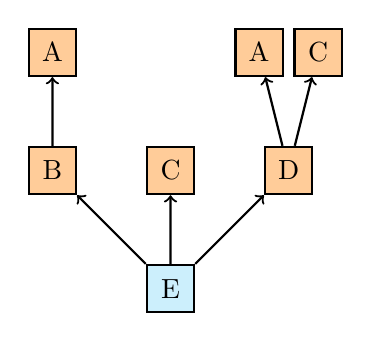
\begin{tikzpicture}[->,thick,
       block/.style={rectangle,draw,fill=cyan!20,minimum size=6mm},
	   comp/.style={rectangle,draw,fill=orange!40, minimum size=6mm},
	   level/.style={sibling distance = 1.5cm/#1, level distance = -1.5cm}]
   \node [block] (a1) {E} 
       child {node [comp] {B}
               child {node [comp] {A}}} 
       child {node [comp] {C}} 
       child {node [comp] {D} 
               child {node [comp] {A}}
               child {node [comp] {C}}};
\end{tikzpicture}
\end{center}


Порядок вызова конструкторов: \texttt{A, B, C, A, C, D, E}.

Деструкторы вызываются в обратном порядке.

Проблемы:
\begin{enumerate}
    \item Дублирование \texttt{A} и \texttt{C}.
    \item Недоступность первого \texttt{C}.
\end{enumerate}

\end{frame}

% % % % % % % % % % % % % % % % % % % % % % % % % % % % % % % % %
\begin{frame}[fragile]{Виртуальное наследование}

\begin{center}
\begin{tikzpicture}[thick,
		block/.style={rectangle,draw,fill=cyan!20,minimum size=6mm,minimum width=1.5cm},
		comp/.style={rectangle,draw,fill=orange!40, minimum size=6mm,minimum width=1.5cm}]
   \node [block] (so)					{Song};
   \node [comp]	 (ly)	[above=of re,xshift=-1cm]	{Lyrics}        edge [<-] (so);
   \node [comp]	 (mu)	[above=of re,xshift=+1cm]	{Music}         edge [<-] (so);
   \node [comp]	 (aw1)	[above=of ly]	            {ArtWork}       edge [<-] (ly);
   \node [comp]	 (aw2)	[above=of mu]	            {ArtWork}       edge [<-] (mu);
\end{tikzpicture}\hspace{2cm}
\begin{tikzpicture}[thick,
		block/.style={rectangle,draw,fill=cyan!20,minimum size=6mm,minimum width=1.5cm},
		comp/.style={rectangle,draw,fill=orange!40, minimum size=6mm,minimum width=1.5cm}]
   \node [block] (so)					            {ElfArcher};
   \node [comp]	 (ly)	[above=of re,xshift=-1cm]	{Elf}        edge [<-] (so);
   \node [comp]	 (mu)	[above=of re,xshift=+1cm]	{Archer}       edge [<-] (so);
   \node<1> [comp]	 (aw1)	[above=of ly,xshift=+1cm]   {Unit}  
        edge [<-] node [color=black,xshift= 6mm] {} (mu)
        edge [<-] node [color=black,xshift=-6mm] {} (ly);
   \node<2> [comp]	 (aw1)	[above=of ly,xshift=+1cm]   {Unit}  
           edge [<-,color=red] node [color=black,xshift= 6mm] {\color{MOOCBlue}{virtual}} (mu)
           edge [<-,color=red] node [color=black,xshift=-6mm] {\color{MOOCBlue}{virtual}} (ly);
\end{tikzpicture}
\end{center}
\pause

    \begin{lstlisting}
struct Unit {};
struct Elf:  virtual Unit {};
struct Archer: virtual Unit {};
struct ElfArcher: Elf, Archer {};
    \end{lstlisting}
\end{frame}

% % % % % % % % % % % % % % % % % % % % % % % % % % % % % % % % %
\begin{frame}[fragile]{Как устроено расположение в памяти?}{}
\vspace{10pt}
\parbox{4cm}{
\begin{tikzpicture}[thick,
		block/.style={rectangle,draw,fill=cyan!20,minimum size=6mm,minimum width=1.5cm},
		comp/.style={rectangle,draw,fill=orange!40, minimum size=6mm,minimum width=1.5cm}]
   \node [block] (so)					            {ElfArcher};
   \node [comp]	 (ly)	[above=of re,xshift=-1cm]	{Elf}        edge [<-] (so);
   \node [comp]	 (mu)	[above=of re,xshift=+1cm]	{Archer}       edge [<-] (so);
   \node [comp]	 (aw1)	[above=of ly,xshift=+1cm]   {Unit}  
        edge [<-,color=red] node [color=black,xshift= 6mm] {\color{MOOCBlue}{virtual}} (mu)
        edge [<-,color=red] node [color=black,xshift=-6mm] {\color{MOOCBlue}{virtual}} (ly);
\end{tikzpicture}}\parbox{6cm}{
\begin{tikzpicture}
    \tikzstyle{every path}=[thick]
    \tikzstyle{tmtape}=[draw,minimum height=6mm, minimum width=1.5cm]
\begin{scope}[start chain=1 going right,node distance=-0.15mm]
    \node [on chain=1,tmtape,draw=none, minimum width=25mm] {Elf};
    \node [on chain=1,tmtape] {Unit};
    \node [on chain=1,tmtape] {Elf};
\end{scope}
\begin{scope}[start chain=1 going right,node distance=-0.15mm,yshift=-1cm]
    \node [on chain=1,tmtape,draw=none, minimum width=25mm] {Archer};
    \node [on chain=1,tmtape] {Unit};
    \node [on chain=1,tmtape] {Archer};
\end{scope}
\begin{scope}[start chain=1 going right,node distance=-0.15mm,yshift=-2cm]
    \node [on chain=1,tmtape,draw=none, minimum width=25mm] {ElfArcher?};
    \node [on chain=1,tmtape] {Unit};
    \node [on chain=1,tmtape] {Elf};
    \node [on chain=1,tmtape] {Archer};
\end{scope}
\begin{scope}[start chain=1 going right,node distance=-0.15mm,yshift=-3cm]
    \node [on chain=1,tmtape,draw=none, minimum width=25mm] {ElfArcher?};
    \node [on chain=1,tmtape] {Elf};
    \node [on chain=1,tmtape] {Unit};
    \node [on chain=1,tmtape] {Archer};
\end{scope}
\end{tikzpicture}}
\vskip5mm\pause

\parbox{4cm}{
На самом деле.}\parbox{6cm}{
\begin{tikzpicture}
    \tikzstyle{every path}=[thick]
    \tikzstyle{tmtape}=[draw,minimum height=6mm, minimum width=1.5cm]
\begin{scope}[start chain=1 going right,node distance=-0.15mm]
    \node [on chain=1,tmtape,draw=none, minimum width=25mm] {Elf};
    \node [on chain=1,tmtape] {Elf};
    \node [on chain=1,tmtape] {Unit};
\end{scope}
\begin{scope}[start chain=1 going right,node distance=-0.15mm,yshift=-1cm]
    \node [on chain=1,tmtape,draw=none, minimum width=25mm] {Archer};
    \node [on chain=1,tmtape] {Archer};
    \node [on chain=1,tmtape] {Unit};
\end{scope}
\begin{scope}[start chain=1 going right,node distance=-0.15mm,yshift=-2cm]
    \tikzstyle{every path}=[thick]
    \tikzstyle{tmtape}=[draw,minimum height=6mm, minimum width=1.5cm]
    \node [on chain=1,tmtape,draw=none, minimum width=25mm] {ElfArcher};
    \node [on chain=1,tmtape] {Elf};
    \node [on chain=1,tmtape] {Archer};
    \node [on chain=1,tmtape] {Unit};
\end{scope}
\end{tikzpicture}}
\end{frame}

% % % % % % % % % % % % % % % % % % % % % % % % % % % % % % % % %
\begin{frame}[fragile]{Доступ через таблицу виртуальных методов}
    \begin{lstlisting}
struct Unit { 
    unitid id;
};
struct Elf  : virtual Unit { };
struct Archer : virtual Unit { };
struct ElfArcher : Elf, Archer { };
    \end{lstlisting}
    \pause
Рассмотрим такой код:
    \begin{lstlisting}
    Elf * e = (rand() % 2)? new Elf() : new ElfArcher();
    unitid id = e->id; // (*)
    \end{lstlisting}
    \pause
Строка \texttt{(*)} будет преобразована в строку
    \begin{lstlisting}
    unitid id = e->__getUnitPtr__()->id;
    \end{lstlisting}
где \texttt{\_\_getUnitPtr\_\_()}~— это служебный виртуальный метод.
\end{frame}


% % % % % % % % % % % % % % % % % % % % % % % % % % % % % % % % %
\begin{frame}[fragile]{Кто вызывает конструктор базового класса?}
\begin{minipage}{.7\textwidth}
    \begin{lstlisting}
struct Unit { 
    Unit(unitid id, int health_points); 
};
struct Elf: virtual Unit {
    explicit Elf(unitid id) 
        : Unit(id, 100) {}
};
struct Archer: virtual Unit {
    explicit Archer(unitid id) 
        : Unit(id, 120) {}
};
struct ElfArcher: Elf, Archer {
    explicit ElfArcher(unitid id) 
        : Unit(id, 150)
        , Elf(id)
        , Archer(id) {}
};
    \end{lstlisting}
\end{minipage}
\begin{minipage}{.25\textwidth}
\begin{tikzpicture}[thick,
		block/.style={rectangle,draw,fill=cyan!20,minimum size=6mm,minimum width=1.5cm},
		comp/.style={rectangle,draw,fill=orange!40, minimum size=6mm,minimum width=1.5cm}]
   \node [block] (so)					            {ElfArcher};
   \node [comp]	 (ly)	[above=of re,xshift=-1cm]	{Elf}        edge [<-] (so);
   \node [comp]	 (mu)	[above=of re,xshift=+1cm]	{Archer}       edge [<-] (so);
   \node [comp]	 (aw1)	[above=of ly,xshift=+1cm]   {Unit}  
           edge [<-,color=red] node [color=black,xshift= 6mm] {\color{MOOCBlue}{virtual}} (mu)
           edge [<-,color=red] node [color=black,xshift=-6mm] {\color{MOOCBlue}{virtual}} (ly);
\end{tikzpicture}
\end{minipage}

\end{frame}

% % % % % % % % % % % % % % % % % % % % % % % % % % % % % % % % %
\begin{frame}[fragile]{Заключение}
    \begin{itemize}
        \item Не используйте множественное наследование для наследования
            реализации.
        
        \pitem Используйте концепцию интерфейсов (классы без реализаций и членов данных).

        \pitem Помните о неприятностях, связанных с множественным наследованием.

        \pitem Хорошо подумайте перед тем, как использовать виртуальное
            наследование.

        \pitem Помните о неприятностях, связанных с виртуальным наследованием.
    \end{itemize}
\end{frame}


% % % % % % % % % % % % % % % % % % % % % % % % % % % % % % % % %
\begin{frame}[fragile]{Множественное наследование}
    \emph{Множественное наследование (multiple inheritance)}~--- возможность
    наследовать сразу несколько классов.
\medskip
    \begin{lstlisting}
struct Unit {
    Unit(unitid id, int hp): id_(id), hp_(hp) {}
    virtual unitid id() const { return id_; }
    virtual int    hp() const { return hp_; }
private:
    unitid id_;
    int	   hp_;
};

struct Elf:    Unit { ... };
struct Archer: Unit { ... };

struct ElfArcher: Elf, Archer {
    unitid id() const { return Elf::id(); }
    int    hp() const { return Elf::hp(); }
};
    \end{lstlisting}
\end{frame}

% % % % % % % % % % % % % % % % % % % % % % % % % % % % % % % % %
\begin{frame}[fragile]{Представление в памяти}
\begin{center}
\begin{tikzpicture}
   \begin{scope}[thick,
       block/.style={rectangle,draw,fill=cyan!20,minimum size=6mm,minimum width=1.3cm},
	   comp/.style={rectangle,draw,fill=orange!40, minimum size=6mm,minimum width=1.3cm}]
   \node [block] (re)	              				{ElfArcher};
   \node [comp]	 (st)	[above=of re,xshift=+1cm]	{Archer} edge [<-] (re);
   \node [comp]	 (em)	[above=of re,xshift=-1cm]	{Elf}  edge [<-] (re);
   \node [comp]	 (p1)	[above=of st]	            {Unit}   edge [<-] (st);
   \node [comp]	 (p2)	[above=of em]	            {Unit}   edge [<-] (em);
   \end{scope}
\end{tikzpicture}\hfill
\begin{tikzpicture}
\begin{scope}[start chain=1 going right,node distance=-0.15mm,yshift=-3cm]
    \tikzstyle{every path}=[thick]
    \tikzstyle{tmtape}=[draw,minimum height=6mm,fill=orange!40,minimum width=1.3cm]
    \node [on chain=1,tmtape] (p1) {Unit};
    \node [on chain=1,tmtape] (st) {Elf};
    \node [on chain=1,tmtape] (p2) {Unit};
    \node [on chain=1,tmtape] (em) {Archer};
    \node [on chain=1,tmtape,fill=cyan!20] (ea) {ElfArcher};
    \node [below=of p1, yshift=-1cm] (s1) {Elf}    edge [->] (p1.south west);
    \node [below=of s1] {ElfArcher};

    \node [below=of p2, yshift=-1cm] {Archer}    edge [->] (p2.south west);
\end{scope}
\end{tikzpicture}
\end{center}

{\bf Важно:} указатели при приведении могут смещаться.

\end{frame}


% % % % % % % % % % % % % % % % % % % % % % % % % % % % % % % % %
\begin{frame}[fragile]{Создание и удаление объекта}
\begin{center}
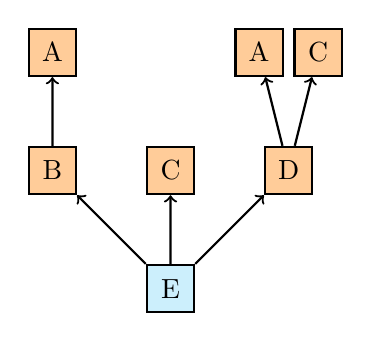
\begin{tikzpicture}[->,thick,
       block/.style={rectangle,draw,fill=cyan!20,minimum size=6mm},
	   comp/.style={rectangle,draw,fill=orange!40, minimum size=6mm},
	   level/.style={sibling distance = 1.5cm/#1, level distance = -1.5cm}]
   \node [block] (a1) {E} 
       child {node [comp] {B}
               child {node [comp] {A}}} 
       child {node [comp] {C}} 
       child {node [comp] {D} 
               child {node [comp] {A}}
               child {node [comp] {C}}};
\end{tikzpicture}
\end{center}


Порядок вызова конструкторов: \texttt{A, B, C, A, C, D, E}.

Деструкторы вызываются в обратном порядке.

Проблемы:
\begin{enumerate}
    \item Дублирование \texttt{A} и \texttt{C}.
    \item Недоступность первого \texttt{C}.
\end{enumerate}

\end{frame}

% % % % % % % % % % % % % % % % % % % % % % % % % % % % % % % % %
\begin{frame}[fragile]{Виртуальное наследование}

\begin{center}
\begin{tikzpicture}[thick,
		block/.style={rectangle,draw,fill=cyan!20,minimum size=6mm,minimum width=1.5cm},
		comp/.style={rectangle,draw,fill=orange!40, minimum size=6mm,minimum width=1.5cm}]
   \node [block] (so)					{Song};
   \node [comp]	 (ly)	[above=of re,xshift=-1cm]	{Lyrics}        edge [<-] (so);
   \node [comp]	 (mu)	[above=of re,xshift=+1cm]	{Music}         edge [<-] (so);
   \node [comp]	 (aw1)	[above=of ly]	            {ArtWork}       edge [<-] (ly);
   \node [comp]	 (aw2)	[above=of mu]	            {ArtWork}       edge [<-] (mu);
\end{tikzpicture}\hspace{2cm}
\begin{tikzpicture}[thick,
		block/.style={rectangle,draw,fill=cyan!20,minimum size=6mm,minimum width=1.5cm},
		comp/.style={rectangle,draw,fill=orange!40, minimum size=6mm,minimum width=1.5cm}]
   \node [block] (so)					            {ElfArcher};
   \node [comp]	 (ly)	[above=of re,xshift=-1cm]	{Elf}        edge [<-] (so);
   \node [comp]	 (mu)	[above=of re,xshift=+1cm]	{Archer}       edge [<-] (so);
   \node<1> [comp]	 (aw1)	[above=of ly,xshift=+1cm]   {Unit}  
        edge [<-] node [color=black,xshift= 6mm] {} (mu)
        edge [<-] node [color=black,xshift=-6mm] {} (ly);
   \node<2> [comp]	 (aw1)	[above=of ly,xshift=+1cm]   {Unit}  
           edge [<-,color=red] node [color=black,xshift= 6mm] {\color{MOOCBlue}{virtual}} (mu)
           edge [<-,color=red] node [color=black,xshift=-6mm] {\color{MOOCBlue}{virtual}} (ly);
\end{tikzpicture}
\end{center}
\pause

    \begin{lstlisting}
struct Unit {};
struct Elf:  virtual Unit {};
struct Archer: virtual Unit {};
struct ElfArcher: Elf, Archer {};
    \end{lstlisting}
\end{frame}

% % % % % % % % % % % % % % % % % % % % % % % % % % % % % % % % %
\begin{frame}[fragile]{Как устроено расположение в памяти?}{}
\vspace{10pt}
\parbox{4cm}{
\begin{tikzpicture}[thick,
		block/.style={rectangle,draw,fill=cyan!20,minimum size=6mm,minimum width=1.5cm},
		comp/.style={rectangle,draw,fill=orange!40, minimum size=6mm,minimum width=1.5cm}]
   \node [block] (so)					            {ElfArcher};
   \node [comp]	 (ly)	[above=of re,xshift=-1cm]	{Elf}        edge [<-] (so);
   \node [comp]	 (mu)	[above=of re,xshift=+1cm]	{Archer}       edge [<-] (so);
   \node [comp]	 (aw1)	[above=of ly,xshift=+1cm]   {Unit}  
        edge [<-,color=red] node [color=black,xshift= 6mm] {\color{MOOCBlue}{virtual}} (mu)
        edge [<-,color=red] node [color=black,xshift=-6mm] {\color{MOOCBlue}{virtual}} (ly);
\end{tikzpicture}}\parbox{6cm}{
\begin{tikzpicture}
    \tikzstyle{every path}=[thick]
    \tikzstyle{tmtape}=[draw,minimum height=6mm, minimum width=1.5cm]
\begin{scope}[start chain=1 going right,node distance=-0.15mm]
    \node [on chain=1,tmtape,draw=none, minimum width=25mm] {Elf};
    \node [on chain=1,tmtape] {Unit};
    \node [on chain=1,tmtape] {Elf};
\end{scope}
\begin{scope}[start chain=1 going right,node distance=-0.15mm,yshift=-1cm]
    \node [on chain=1,tmtape,draw=none, minimum width=25mm] {Archer};
    \node [on chain=1,tmtape] {Unit};
    \node [on chain=1,tmtape] {Archer};
\end{scope}
\begin{scope}[start chain=1 going right,node distance=-0.15mm,yshift=-2cm]
    \node [on chain=1,tmtape,draw=none, minimum width=25mm] {ElfArcher?};
    \node [on chain=1,tmtape] {Unit};
    \node [on chain=1,tmtape] {Elf};
    \node [on chain=1,tmtape] {Archer};
\end{scope}
\begin{scope}[start chain=1 going right,node distance=-0.15mm,yshift=-3cm]
    \node [on chain=1,tmtape,draw=none, minimum width=25mm] {ElfArcher?};
    \node [on chain=1,tmtape] {Elf};
    \node [on chain=1,tmtape] {Unit};
    \node [on chain=1,tmtape] {Archer};
\end{scope}
\end{tikzpicture}}
\vskip5mm\pause

\parbox{4cm}{
На самом деле.}\parbox{6cm}{
\begin{tikzpicture}
    \tikzstyle{every path}=[thick]
    \tikzstyle{tmtape}=[draw,minimum height=6mm, minimum width=1.5cm]
\begin{scope}[start chain=1 going right,node distance=-0.15mm]
    \node [on chain=1,tmtape,draw=none, minimum width=25mm] {Elf};
    \node [on chain=1,tmtape] {Elf};
    \node [on chain=1,tmtape] {Unit};
\end{scope}
\begin{scope}[start chain=1 going right,node distance=-0.15mm,yshift=-1cm]
    \node [on chain=1,tmtape,draw=none, minimum width=25mm] {Archer};
    \node [on chain=1,tmtape] {Archer};
    \node [on chain=1,tmtape] {Unit};
\end{scope}
\begin{scope}[start chain=1 going right,node distance=-0.15mm,yshift=-2cm]
    \tikzstyle{every path}=[thick]
    \tikzstyle{tmtape}=[draw,minimum height=6mm, minimum width=1.5cm]
    \node [on chain=1,tmtape,draw=none, minimum width=25mm] {ElfArcher};
    \node [on chain=1,tmtape] {Elf};
    \node [on chain=1,tmtape] {Archer};
    \node [on chain=1,tmtape] {Unit};
\end{scope}
\end{tikzpicture}}
\end{frame}

% % % % % % % % % % % % % % % % % % % % % % % % % % % % % % % % %
\begin{frame}[fragile]{Доступ через таблицу виртуальных методов}
    \begin{lstlisting}
struct Unit { 
    unitid id;
};
struct Elf  : virtual Unit { };
struct Archer : virtual Unit { };
struct ElfArcher : Elf, Archer { };
    \end{lstlisting}
    \pause
Рассмотрим такой код:
    \begin{lstlisting}
    Elf * e = (rand() % 2)? new Elf() : new ElfArcher();
    unitid id = e->id; // (*)
    \end{lstlisting}
    \pause
Строка \texttt{(*)} будет преобразована в строку
    \begin{lstlisting}
    unitid id = e->__getUnitPtr__()->id;
    \end{lstlisting}
где \texttt{\_\_getUnitPtr\_\_()}~— это служебный виртуальный метод.
\end{frame}


% % % % % % % % % % % % % % % % % % % % % % % % % % % % % % % % %
\begin{frame}[fragile]{Кто вызывает конструктор базового класса?}
\begin{minipage}{.7\textwidth}
    \begin{lstlisting}
struct Unit { 
    Unit(unitid id, int health_points); 
};
struct Elf: virtual Unit {
    explicit Elf(unitid id) 
        : Unit(id, 100) {}
};
struct Archer: virtual Unit {
    explicit Archer(unitid id) 
        : Unit(id, 120) {}
};
struct ElfArcher: Elf, Archer {
    explicit ElfArcher(unitid id) 
        : Unit(id, 150)
        , Elf(id)
        , Archer(id) {}
};
    \end{lstlisting}
\end{minipage}
\begin{minipage}{.25\textwidth}
\begin{tikzpicture}[thick,
		block/.style={rectangle,draw,fill=cyan!20,minimum size=6mm,minimum width=1.5cm},
		comp/.style={rectangle,draw,fill=orange!40, minimum size=6mm,minimum width=1.5cm}]
   \node [block] (so)					            {ElfArcher};
   \node [comp]	 (ly)	[above=of re,xshift=-1cm]	{Elf}        edge [<-] (so);
   \node [comp]	 (mu)	[above=of re,xshift=+1cm]	{Archer}       edge [<-] (so);
   \node [comp]	 (aw1)	[above=of ly,xshift=+1cm]   {Unit}  
           edge [<-,color=red] node [color=black,xshift= 6mm] {\color{MOOCBlue}{virtual}} (mu)
           edge [<-,color=red] node [color=black,xshift=-6mm] {\color{MOOCBlue}{virtual}} (ly);
\end{tikzpicture}
\end{minipage}

\end{frame}

% % % % % % % % % % % % % % % % % % % % % % % % % % % % % % % % %
\begin{frame}[fragile]{Заключение}
    \begin{itemize}
        \item Не используйте множественное наследование для наследования
            реализации.
        
        \pitem Используйте концепцию интерфейсов (классы без реализаций и членов данных).

        \pitem Помните о неприятностях, связанных с множественным наследованием.

        \pitem Хорошо подумайте перед тем, как использовать виртуальное
            наследование.

        \pitem Помните о неприятностях, связанных с виртуальным наследованием.
    \end{itemize}
\end{frame}
\end{document}
